The research will apply and extend the latest release series of the \gls{cesm} and its components, \gls{clm}~5 including \gls{bvoc} emissions (\gls{megan} model \parencite{ACP:Guenther2006}, \gls{cam}~6 with online (super-fast) chemistry (\gls{impact} model, \textcite{JGR:Rotman2004}). Below, we provide  a brief technical account of the model components of \gls{cesm} most relevant to the planned work, \gls{clm} including \gls{megan}, and \gls{cam}. Subsequently we review  the Lombardozzi model of ozone damage and close by introducing the new process oriented plant physiological model of ozone damage, developed by the applicant, including the planned integration into \gls{clm} that stands at the core of the \gls{odina} project.

\begin{wrapfigure}[31]{L}[0pt]{0.5\textwidth}
  % R - floating; r - h! [narrow lines] <- reduce whitespace below [17]
  \centering
  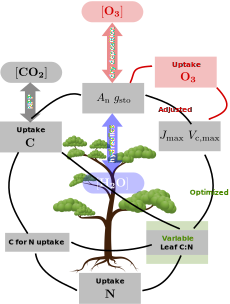
\includegraphics[width=0.48\textwidth]{ozone_luna_scheme}
  \caption{Schematic view of \gls{odina} model integration into \gls{clm}~5. Round boxes represent affected tropospheric chemistry (\gls{cam}-chem) and trace gas concentrations, e.g. \ch{[CO_2]}, \ch{[O_3]}, \ch{[H_2O]}. Annotated arrows denote associated process. Squared boxes represent processes in the land model (\gls{clm}). Plants {\color{darkgray}invest carbon} to {\color{darkgray}take up nutrients}. A variable \ch{C:N} ratio at leaf level steers the optimization of electron transport ($\mathrm{J_{max}}$) and carboxylation rate ($\mathrm{V_{cmax}}$), which determine photosynthesis ($\mathrm{A_n}$) and stomatal conductance ($\mathrm{g_{sto}}$). $\mathrm{g_{sto}}$ controls transpiration and thus {\color{blue}plant hydraulics}. {\color{red}Ozone uptake} is determined by $\mathrm{g_{sto}}$ and reduces both $\mathrm{J_{max}}$ and $\mathrm{V_{cmax}}$.
}
  \label{fig:ozone_odina}
\end{wrapfigure}

\section{\gls{cesm}}
\label{sec:cesm}
In \gls{clm}~5, \textbf{photosynthesis} (and hence the {\color{darkgray}carbon cycle}) is tied to \textbf{\color{darkgray}plant nutrient dynamics} (dark gray boxes in Fig.~\ref{fig:ozone_odina}) which incorporates the \textbf{\gls{fun}} model \parencites{GBC:Fisher2010}{JGR:Brzostek2014}{GCB:Shi2015}. The concept of \gls{fun} is that nitrogen uptake requires an investment of energy (e.g. carbon) and that there is a large number of potential sources of nitrogen available in the environment. The ratio of carbon invested to acquire nitrogen is therefore treated as a cost in the model. \gls{fun} calculates the rate of symbiotic nitrogen fixation for nitrogen that is passed directly to the plant, and subsequently delivered and incorporated  as inorganic ammonium in the soil \parencite{GBC:Cleveland1999}, separately. Nutrient limitation is represented by a variable plant \ch{C:N} ratio which allows plants to adjust their \ch{C:N} ratio at the leaf level at the cost of nitrogen \parencite{JAMES:Ghimire2016}. The \textbf{\gls{luna}} model \parencites{STE:Xu2019}{GMD:Ali2016} finally links these processes with photosynthesis. To this end the \gls{luna} model calculates the photosynthetic capacity based on optimization of the use of leaf nitrogen under different environmental conditions. \textbf{Stomatal conductance} is based on this \textbf{nitrogen-limited photosynthesis} rather than on potential photosynthesis. The maximum stomatal conductance is obtained from the \textbf{Medlyn stomatal conductance} model \parencite{GCB:Medlyn2011} which is preferred over Ball-Berry-type models \parencite{BallBerry1987} for it’s more realistic behavior at low humidity levels (high vapor pressure deficit) \parencites{PR:Rogers2013}{NP:Rogers2017}.

As a \textbf{plant hydraulic stress} routine explicitly models water transport through the vegetation according to a simple hydraulic framework \parencite{JAMES:Kennedy2019}, stomatal conductance is also a function of prognostic leaf water potential and hence forced by transpiration. Plant water stress is calculated as the ratio of attenuated stomatal conductance to maximum stomatal conductance.

\textbf{Biogenic emissions} from vegetation are not directly integrated into the modelling framework described above but handled by \gls{megan} \parencite{ACP:Guenther2006}. \gls{megan} uses above canopy atmospheric forcing, e.g. solar radiation, temperature, and moisture, and \ch{[CO_2]} as input variables. \gls{megan} receives only \gls{lai} as vegetation input information, which can be either prescribed (\gls{sp} mode) or dynamic (\gls{bgc} mode) and \gls{pft}. In \gls{clm}~5, \gls{megan}~version~2.1 \parencite{GMD:Guenther2012} is implemented. \gls{megan}~2.1 includes 147 chemical compounds which can be subset and grouped together (e.g. \emph{isoprene} = pentane + hexane + heptane + tricyclene). In \gls{clm}, trapping of emissions inside of the canopy is explicitly disabled (i.e., escape efficiency set to 1).

In \textbf{\gls{cam}-chem}, \textbf{dry deposition} follows the resistance approach originally described by \textcites{AE:Wesely1989}{AE:Walcek1986} and updated sequentially \parencites{AE:Walmsley1996}{AE:Wesely2000}. All deposited chemical species are mapped to a weighted-combination of ozone and sulfur dioxide depositions to characterize their oxidation potential versus their solubility in water which is dependent on the effective Henry’s law coefficient of the species. All species in the mechanism are per default affected by dry deposition if deposition velocities are defined. The computation of \textbf{deposition velocities} (or resistances) ties \gls{cam}-chem to \gls{clm}. Dry deposition velocities vary with \gls{pft}. A grid-averaged velocity is computed as the weighted-mean over all land cover types. The impact from changes in land cover, land use or climate are thus directly reflected in the coupled model \parencite{GMD:Lamarque2012}. 

\section{Ozone damage}
\label{sec:ozone_damage}
\textbf{At present, ozone damage on vegetation is not reliably accounted for in \gls{cesm}}. There are a couple of technical reasons for this. First of all, the land surface model (\gls{clm}) as a stand-alone model would need at least a reliable global climatology to integrate ozone damage in its default setup. Global ozone reanalysis (i.e. \gls{cam} reanalysis products of \gls{ecmwf}) or satellite derived tropospheric ozone would be candidates but show, despite improvements in recent years, considerable biases compared to observations \textbf{TODO: Add reference https://gmd.copernicus.org/articles/13/1513/2020/}. Though ozone climatologies based on older \gls{cesm} runs with \gls{cam} and \gls{clm} exist \parencite{ACP:Lamarque2010}. Common caveat of such simulations with uncoupled ozone are
\begin{enumerate}
\itemsep0pt
\item inconsistency between the land surface (e.g. land use type, roughness length) used in the \gls{ccm} and the uncoupled land surfaces model with ozone damage functions, and
\item ozone concentrations are not provided to \gls{clm} directly from the atmosphere and therefore mostly not in agreement with atmospheric abundances.
\end{enumerate}

\textbf{Ozone damage in \gls{clm}~5} is based on the work of Lombardozzi \textcite{Oe:Lombardozzi2012} which showed an effective decoupling of $A_\mathrm{n}$ and $g_\mathrm{sto}$ under high \gls{cuo}, with $g_\mathrm{sto}$ being less sensitive to cumulative uptake of ozone. If taken into consideration this improves global projections of \gls{gpp} and transpiration considerably \parencite{BGS:Lombardozzi2012}, especially in tropical regions as also shown by \textcite{Nat:Sitch2007} and \textcite{ACP:Pacifico2015}. In this implementation, damage coefficients for $g_\mathrm{sto}$ and $A_\mathrm{n}$ are defined for coniferous, deciduous, and non-woody \glspl{pft}, respectively. \gls{cuo} can be regulated through an uptake threshold $\Phi_\mathrm{th}$, further a healing factor is computed based on change in \gls{lai} (growth of new leaves). \textbf{Added text: Technical limitations and issues of the current ozone damage module include its disconnection from the nutrient and carbon cost driven photosynthesis and compatibility with the plant hydraulic module. In particular, the order in which stomatal conductance is reduced under combined thermal and oxidative stress is not clearly constrained.} 

\textbf{Added text:Recent model development efforts led by the applicant have addressed some of the limitations listed above by integrating ozone damage on the process-level. A linear linear relationship between \gls{cuo} and $\mathrm{J_{max}}$ in forced and control experiments was deduced based on the body of peer reviewed research articles published in recent years.} The \gls{odina} model integrates seamlessly into existing, scientifically validated modules in \gls{clm} (e.g. \gls{fun}, \gls{luna}). The integration of \gls{odina} into the existing framework of \gls{clm}~5 is schematically illustrated in Fig.~\ref{fig:ozone_odina}. \gls{odina} also builds on previous efforts by \textcites{BGS:Lombardozzi2012}{Oe:Lombardozzi2012}, leading to a comprehensive database of experimental data of ozone damage and an implementation of an ozone damage module in \gls{clm}~4 \parencite{BGS:Lombardozzi2013}. This database will be used for model evaluation of \gls{odina} as data are not included in the derivation of the linear relationship detailed above. One of the advantages of the \gls{odina} model is that it can be used to study ozone effects on the \ch{C:N} ratio and thus \textbf{TODO: Add meaning if C:N ratio for plants}. The purpose of this project is to establish the coupling of \gls{clm}~5 to \gls{cam}-chem with respect to ozone through dry deposition and evaluate the comprehensive two-way coupling of ozone-vegetation in the light of progressing climate change.
